% 2011 年北京卷理科第 16 题：四棱锥 P-ABCD。
% 来源 PDF：普通高考/2011/2011北京理.pdf，SHA-256 79351b2b5d5afd29a2d46d50526284443edad4deb64fbaf841db31ce2570c311。
% 原页：第 1 页（A3 三栏）第 3 栏下部，书页码 647。
% 重绘依据：照原页拓扑——P 在 A 正上方，PA 竖直；底面 ABCD 画成平行四边形，
%   A 在最左、B 在前下、C 在最右、D 在后上。实线 PA、PB、PC、PD、AB、BC、CD，
%   虚线 AD、AC、BD。不按比例。
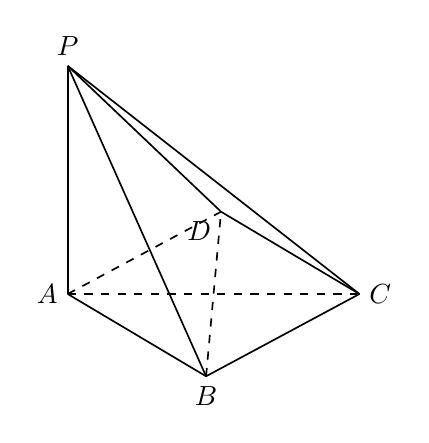
\begin{tikzpicture}[>=stealth, semithick, scale=0.95]
  \coordinate (A) at (0,0);
  \coordinate (B) at (1.85,-1.1);
  \coordinate (C) at (3.9,0);
  \coordinate (D) at (2.05,1.1);
  \coordinate (P) at (0,3.05);

  % 实线
  \draw (P) -- (A);
  \draw (P) -- (B);
  \draw (P) -- (C);
  \draw (P) -- (D);
  \draw (A) -- (B);
  \draw (B) -- (C);
  \draw (C) -- (D);
  % 虚线（被遮挡的棱与对角线）
  \draw[dashed] (A) -- (D);
  \draw[dashed] (A) -- (C);
  \draw[dashed] (B) -- (D);

  \node[above] at (P) {$P$};
  \node[left] at (A) {$A$};
  \node[below] at (B) {$B$};
  \node[right] at (C) {$C$};
  \node[below left] at (D) {$D$};
\end{tikzpicture}
